\documentclass[pdflatex,ja=standard,fleqn]{bxjsarticle}
\usepackage{ascmac,amsmath,amssymb,type1cm,graphicx,booktabs}
\title{情報計算科学レポート2}
\author{J4-210447 川村朋広}
\begin{document}
\maketitle
\section*{(1)}
微分方程式
\begin{eqnarray*}
    \frac{d^2u}{dx^2}=0\quad
    u(0)=0\quad
    u(1)=0
\end{eqnarray*}
の解を求める。\\
【解答】\\
$C_{1}\in\mathbb{R}$として、
\begin{eqnarray*}
    \frac{du}{dx}=C_{1}
\end{eqnarray*}
と置ける。またこれより、$C_{2}\in\mathbb{R}$を用いて
\begin{eqnarray*}
    u(x)=C_{1}x+C_{2}
\end{eqnarray*}
と表される。境界条件より、
\begin{eqnarray*}
    C_{1}=1\quad
    C_{2}=0
\end{eqnarray*}
とわかるので、$u(x)=x$である。
\section*{(2),(3),(4)}
ともに次のページのようなグラフとなり、理論解と一致した。なお(4)について、ノード番号順にx座標を格納した配列を用意した結果、ソースコードに変更を加えなくても、同じ結果を返した。
\begin{figure}[htbp]
    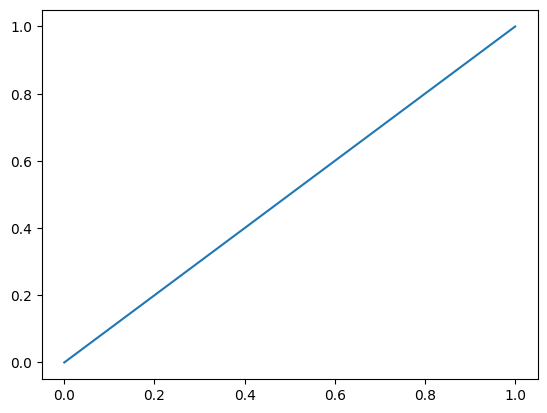
\includegraphics{output.png}
\end{figure}
\end{document}